\begin{figure*}[!t]
\centering
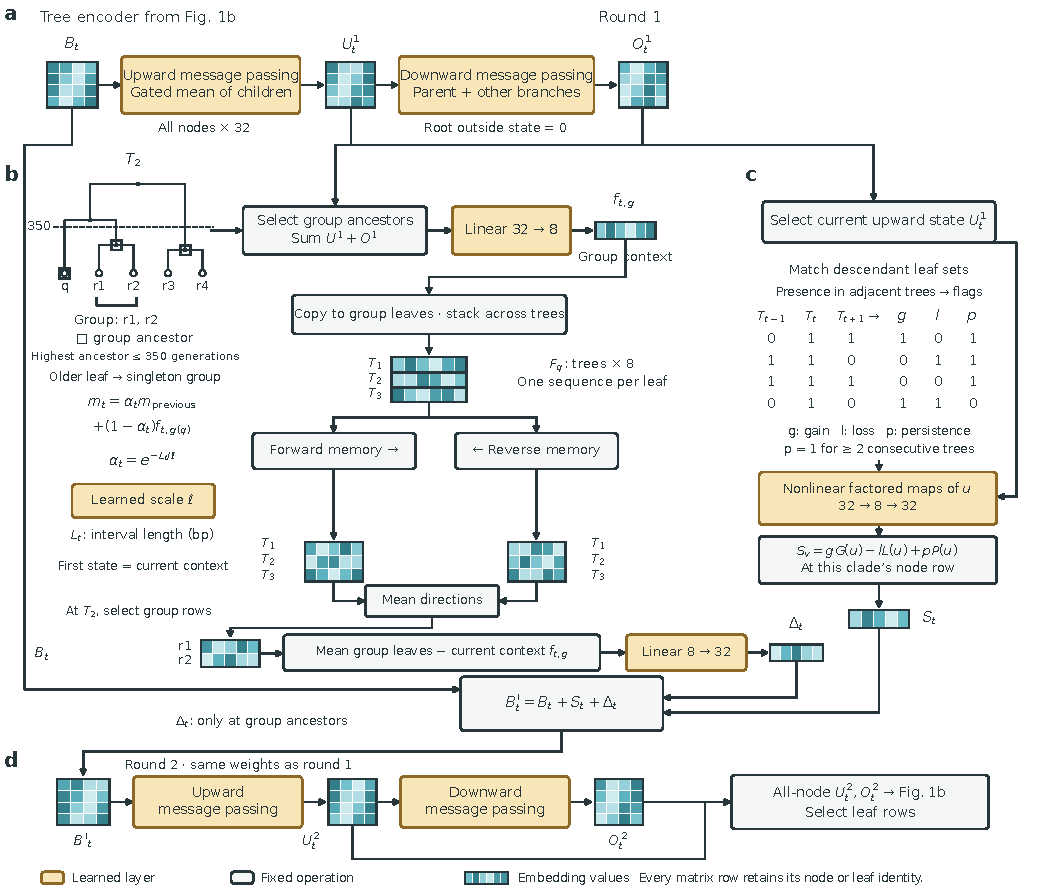
\includegraphics[width=\textwidth]{figures/TreeLoom_encoder.pdf}
\caption{Expansion of the encoder in Figure~\ref{fig:architecture}b. \textbf{a,} Shared upward and downward tree passes run before and after summing the two corrections with the original node embeddings. \textbf{b,} Clade presence and the current upward state produce a structural correction. \textbf{c,} A fixed ancestral age partitions leaves into groups, which supply context from both directional states. Memory follows each leaf across intervals, then averages within current groups. The group correction subtracts the local group context before projection and returns to the current representative. The example follows $r1$ through groups $d,b,b$.}
\label{fig:encoder}
\end{figure*}
